\documentclass[aspectratio=169,10pt]{beamer}
\usetheme{Madrid}
\usecolortheme{seahorse}

\usepackage{amsmath,amssymb,amsfonts}
\usepackage{mathtools}
\usepackage{xcolor}
\usepackage{listings}
\usepackage{graphicx}
\usepackage{array}
\usepackage{xfrac}
\usepackage{fancybox}

\setbeamertemplate{footline}[frame number]
\setbeamertemplate{navigation symbols}{}

\graphicspath{{figures/}}

% Code styling
\lstset{
    language=Python,
    basicstyle=\ttfamily\scriptsize,
    keywordstyle=\color{blue}\bfseries,
    commentstyle=\color{green!50!black}\itshape,
    stringstyle=\color{red},
    breaklines=true,
    frame=single,
    numbers=left,
    numberstyle=\tiny,
    stepnumber=1,
    showstringspaces=false,
    tabsize=2
}

\title{Multivalued Mappings \& Fixed Points}
\subtitle{Chapter 5.4: Fixed Point Theorems for Multifunctions}
\author{Based on Pathak's Introduction to Nonlinear Analysis}
\institute{Fixed Point Theory Course}
\date{\today}

\begin{document}

\frame{\titlepage}

% ============================================================================
% TABLE OF CONTENTS
% ============================================================================

\begin{frame}
\frametitle{Outline}
\tableofcontents
\end{frame}

% ============================================================================
% SECTION 1: INTRODUCTION TO MULTIVALUED MAPPINGS
% ============================================================================

\section{Introduction to Multivalued Mappings}

\begin{frame}
\frametitle{What is a Multivalued Mapping?}

\begin{definition}
A \textbf{multivalued mapping} (or \textbf{multifunction}) is a map
\[
T: X \to 2^X
\]
that assigns to each point $x \in X$ a \textbf{set} $T(x) \subseteq X$
rather than a single point.
\end{definition}

\vspace{0.3cm}

\centering
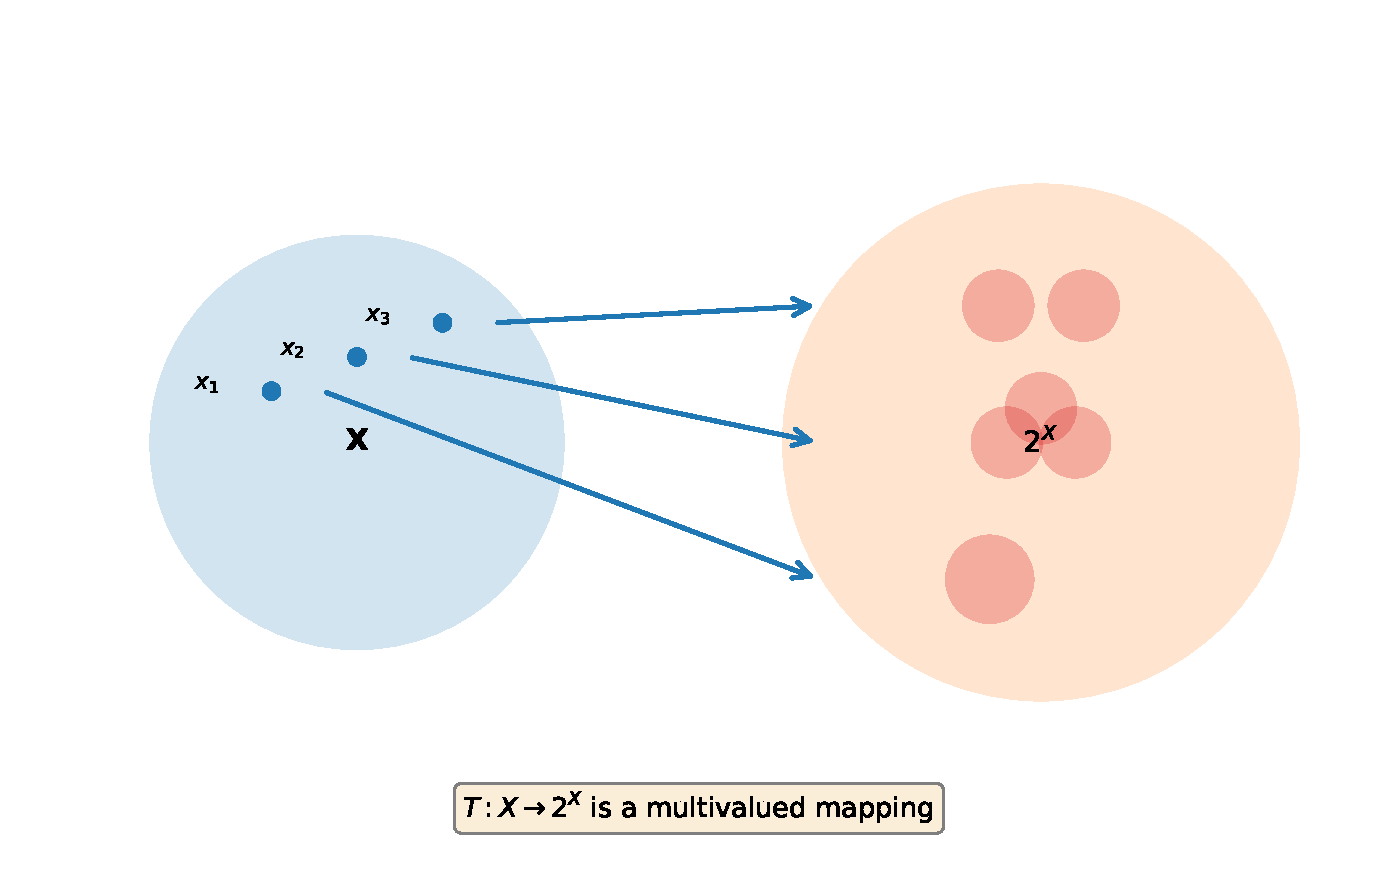
\includegraphics[width=0.7\textwidth]{multivalued_mapping}

\begin{itemize}
    \item Domain: Single points in $X$
    \item Codomain: Subsets of $X$ (power set $2^X$)
    \item Each point maps to a \textbf{set} of values
\end{itemize}

\end{frame}

\begin{frame}
\frametitle{Notation and Basic Concepts}

\begin{itemize}
    \item \textbf{Domain:} $D(T) = \{x \in X : T(x) \neq \emptyset\}$

    \item \textbf{Range:} $R(T) = \bigcup_{x \in D(T)} T(x)$

    \item \textbf{Graph:} $\text{Gr}(T) = \{(x,y) : y \in T(x)\}$

    \item \textbf{Inverse:} $T^{-1}(B) = \{x \in X : T(x) \cap B \neq \emptyset\}$
\end{itemize}

\vspace{0.5cm}

\begin{block}{Example}
Let $X = \mathbb{R}$ and define $T(x) = [x-1, x+1]$. Then:
\begin{itemize}
    \item $D(T) = \mathbb{R}$ (entire domain)
    \item $T(0) = [-1, 1]$, $T(2) = [1, 3]$
    \item Each point maps to an interval
\end{itemize}
\end{block}

\end{frame}

\begin{frame}
\frametitle{Fixed Points for Multivalued Mappings}

\begin{definition}
A point $x_0 \in X$ is a \textbf{fixed point} of the multivalued mapping $T: X \to 2^X$ if
\[
x_0 \in T(x_0)
\]
\end{definition}

\vspace{0.3cm}

\textbf{Key Difference from Single-Valued Case:}
\begin{itemize}
    \item For single-valued $f: X \to X$: fixed point satisfies $f(x_0) = x_0$
    \item For multivalued $T: X \to 2^X$: fixed point satisfies $x_0 \in T(x_0)$
    \item Set membership instead of equality
\end{itemize}

\vspace{0.3cm}

\begin{example}
For $T(x) = [x-1, x+1]$:
\begin{itemize}
    \item Is $x = 0$ a fixed point? Need $0 \in [-1, 1]$. \textcolor{green!50!black}{\checkmark Yes!}
    \item Is $x = 3$ a fixed point? Need $3 \in [2, 4]$. \textcolor{green!50!black}{\checkmark Yes!}
    \item Is $x = 10$ a fixed point? Need $10 \in [9, 11]$. \textcolor{green!50!black}{\checkmark Yes!}
\end{itemize}
\end{example}

\end{frame}

\begin{frame}
\frametitle{Historical Development}

\begin{itemize}
    \item \textbf{1941}: Kakutani proved fixed point theorem for multivalued mappings in $\mathbb{R}^n$

    \item \textbf{1950}: Bohnenblust \& Karlin extended to infinite-dimensional Banach spaces

    \item \textbf{1952}: Fan generalized result to locally convex spaces

    \item \textbf{1969}: Nadler Jr. developed theory of multivalued contractions with Hausdorff metric

    \item \textbf{1970s}: Assad, Kirk, Markin, Smithson advanced theory further
\end{itemize}

\vspace{0.3cm}

\textbf{Applications:}
\begin{itemize}
    \item Control theory and differential equations
    \item Game theory and economics
    \item Variational inequalities
    \item Differential inclusions
\end{itemize}

\end{frame}

% ============================================================================
% SECTION 2: HAUSDORFF-POMPEU METRIC
% ============================================================================

\section{Hausdorff-Pompeu Metric}

\begin{frame}
\frametitle{Measuring Distance Between Sets}

To study contractive multivalued mappings, we need a metric on \textbf{sets}, not just points.

\vspace{0.3cm}

\begin{definition}
Let $(X,d)$ be a metric space. For non-empty sets $A, B \subseteq X$, define:

\begin{align*}
d(a, B) &= \inf_{b \in B} d(a,b) \quad \text{(distance from point to set)} \\[0.2cm]
\rho(A, B) &= \sup_{a \in A} d(a, B) \quad \text{(directed Hausdorff distance)} \\[0.2cm]
H(A, B) &= \max\{\rho(A,B), \rho(B,A)\} \quad \text{(Hausdorff metric)}
\end{align*}
\end{definition}

\vspace{0.2cm}

\begin{block}{Alternative Definition}
\[
H(A,B) = \inf\{\varepsilon > 0 : A \subseteq N(\varepsilon, B) \text{ and } B \subseteq N(\varepsilon, A)\}
\]
where $N(\varepsilon, C) = \{x \in X : d(x,c) < \varepsilon \text{ for some } c \in C\}$
\end{block}

\end{frame}

\begin{frame}
\frametitle{Hausdorff-Pompeu Metric Visualization}

\centering
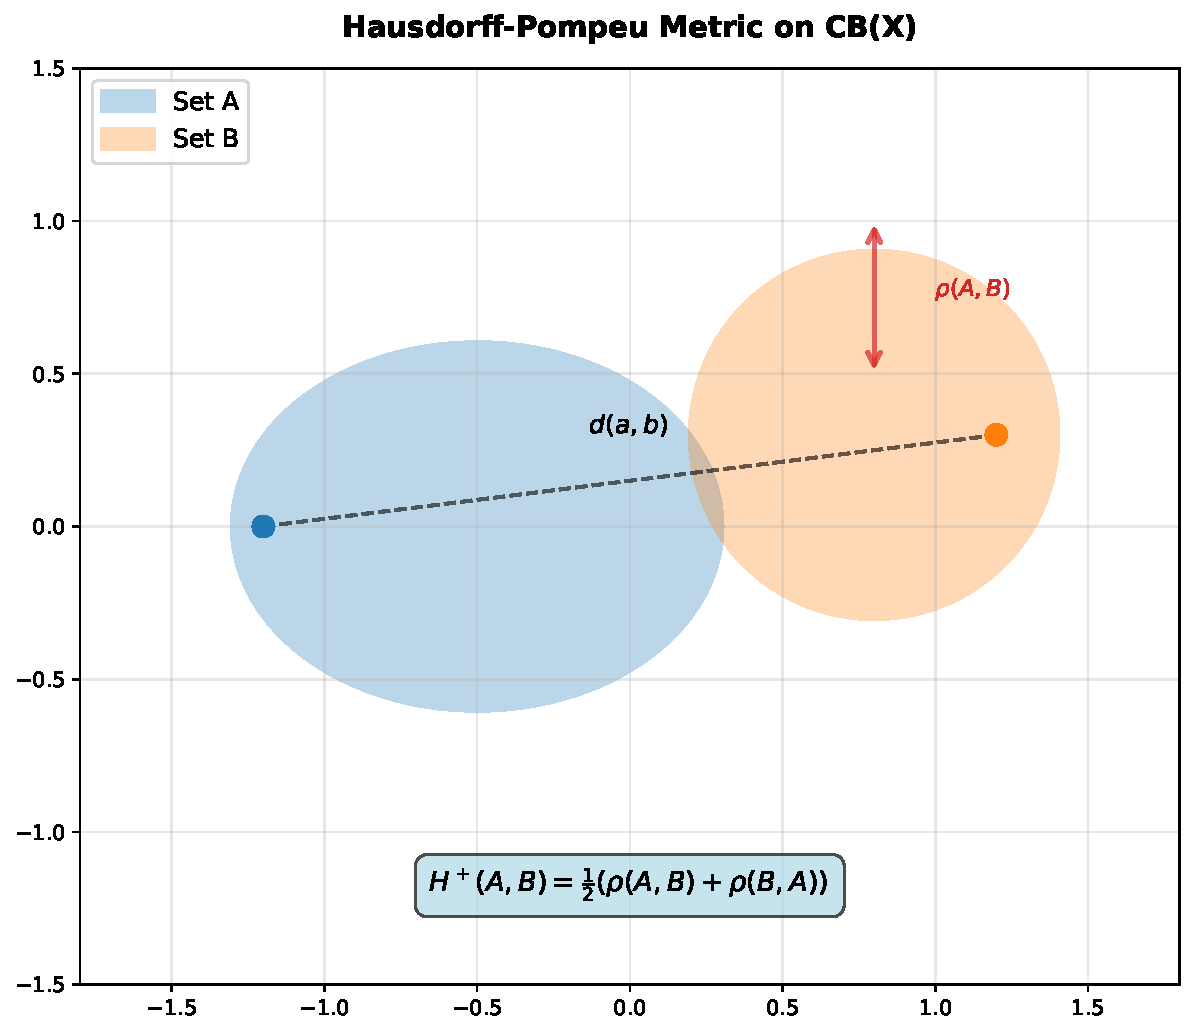
\includegraphics[width=0.8\textwidth]{hausdorff_metric}

\begin{itemize}
    \item $\rho(A,B)$: Maximum distance from any point in $A$ to the set $B$
    \item $H(A,B)$: The maximum of $\rho(A,B)$ and $\rho(B,A)$
    \item Measures how far apart two sets are
\end{itemize}

\end{frame}

\begin{frame}
\frametitle{Properties of the Hausdorff-Pompeu Metric}

\begin{theorem}
Let $(X,d)$ be a complete metric space. Then:
\begin{enumerate}
    \item $(CB(X), H)$ is a complete metric space, where $CB(X)$ is the set of nonempty closed bounded subsets
    \item $K(X)$ (nonempty compact subsets) is a closed subspace of $CB(X)$
    \item For single points: $H(\{a\}, \{b\}) = d(a,b)$
\end{enumerate}
\end{theorem}

\vspace{0.2cm}

\begin{block}{Key Observations}
\begin{itemize}
    \item The Hausdorff metric depends on the underlying metric $d$ on $X$
    \item Two equivalent metrics on $X$ may not generate equivalent Hausdorff metrics
    \item The completeness of $(X,d)$ ensures completeness of $(CB(X), H)$
\end{itemize}
\end{block}

\end{frame}

% ============================================================================
% SECTION 3: CONTINUITY OF MULTIVALUED MAPPINGS
% ============================================================================

\section{Continuity of Multivalued Mappings}

\begin{frame}
\frametitle{Upper Semicontinuity}

\begin{definition}
A multifunction $T: X \to 2^Y$ is \textbf{upper semicontinuous (u.s.c.)} if:
\[
\text{For each closed set } B \subseteq Y, \quad T^{-1}(B) = \{x : T(x) \cap B \neq \emptyset\} \text{ is closed}
\]
\end{definition}

\vspace{0.3cm}

\textbf{Equivalent characterization:}
For each $x \in X$ and open set $U \supseteq T(x)$, there exists an open neighborhood $V$ of $x$ such that $U \supseteq T(y)$ for all $y \in V$.

\vspace{0.3cm}

\centering
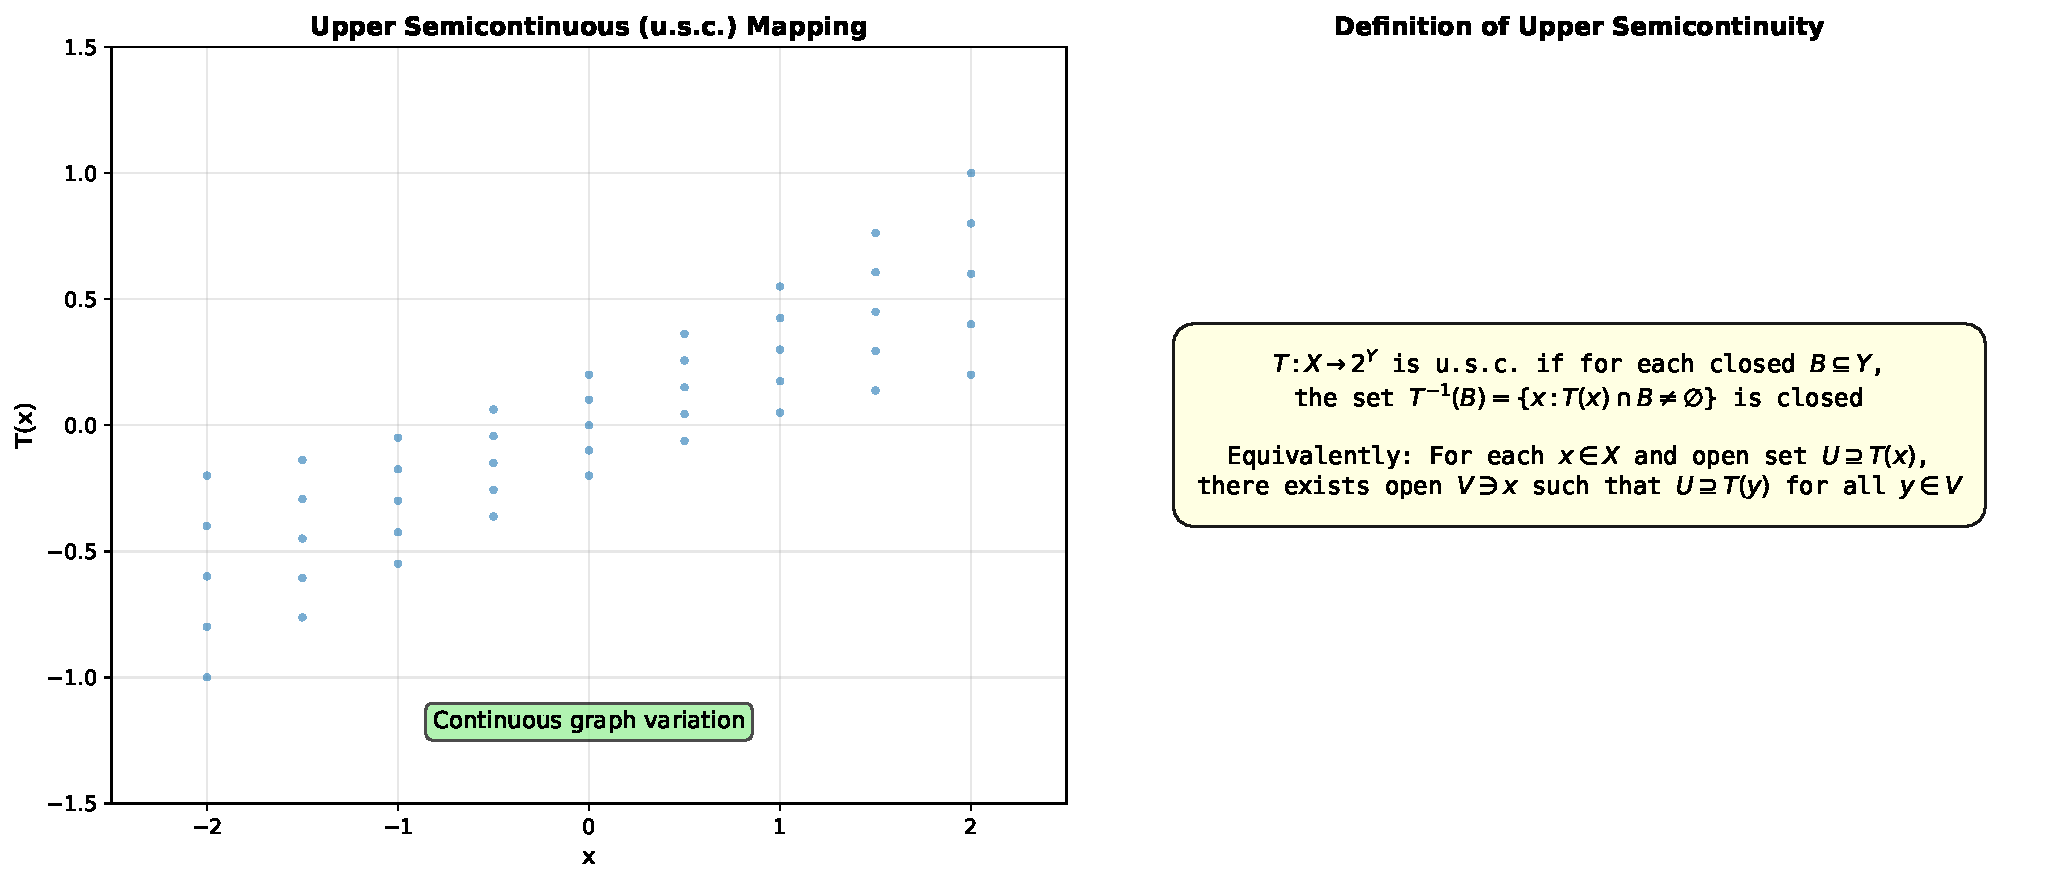
\includegraphics[width=0.9\textwidth]{upper_semicontinuous}

\end{frame}

\begin{frame}
\frametitle{Lower Semicontinuity and Other Notions}

\begin{definition}
A multifunction $T: X \to 2^Y$ is \textbf{lower semicontinuous (l.s.c.)} if:
\[
\text{For each open set } U \subseteq Y, \quad \{x : T(x) \cap U \neq \emptyset\} \text{ is open}
\]
\end{definition}

\vspace{0.3cm}

A multifunction is \textbf{continuous} if it is both u.s.c. and l.s.c.

\vspace{0.3cm}

\begin{block}{Additional Concepts}
\begin{itemize}
    \item \textbf{Point closed:} $T(x)$ is closed for all $x$
    \item \textbf{Point compact:} $T(x)$ is compact for all $x$
    \item \textbf{Point convex:} $T(x)$ is convex for all $x$
\end{itemize}
\end{block}

\vspace{0.3cm}

\textbf{Remark:} Upper semicontinuity is the most natural generalization of continuity for multifunctions.

\end{frame}

% ============================================================================
% SECTION 4: FAN'S AND HIMMELBERG'S THEOREMS
% ============================================================================

\section{Fan's and Himmelberg's Fixed Point Theorems}

\begin{frame}
\frametitle{Fan's Fixed Point Theorem}

\begin{theorem}[Fan, 1952]
Let $X$ be a normed linear space, $K$ a nonempty, compact and convex subset of $X$.
Let $T: K \to 2^K$ be a multifunction such that:
\begin{enumerate}
    \item For each $x \in K$: $T(x)$ is nonempty, closed, and convex
    \item $T$ is upper semicontinuous
\end{enumerate}
Then there exists a fixed point $x^* \in K$ such that $x^* \in T(x^*)$.
\end{theorem}

\vspace{0.3cm}

\textbf{Key Features:}
\begin{itemize}
    \item Generalizes Kakutani's theorem from $\mathbb{R}^n$ to normed spaces
    \item Works in locally convex spaces
    \item No contraction property needed—only compactness and convexity
    \item Purely topological argument
\end{itemize}

\end{frame}

\begin{frame}
\frametitle{Himmelberg's Generalization}

\begin{theorem}[Himmelberg, 1972]
Let $K_1$ be a nonempty and convex subset of a normed linear space $X$.
Let $T: K_1 \to 2^{K_1}$ be a multifunction such that:
\begin{enumerate}
    \item $T$ is upper semicontinuous
    \item For each $x \in K_1$: $T(x)$ is closed and convex
    \item $T(K_1) \subseteq C$ for some compact $C \subseteq K_1$
\end{enumerate}
Then $T$ has a fixed point in $K_1$.
\end{theorem}

\vspace{0.3cm}

\textbf{Improvement over Fan's Theorem:}
\begin{itemize}
    \item Allows non-compact $K_1$
    \item Only requires that $T(K_1)$ be contained in a compact subset
    \item Proof uses topological degree theory
\end{itemize}

\end{frame}

\begin{frame}
\frametitle{Min-Max Theorem}

\begin{theorem}[Consequence of Himmelberg's Theorem]
Let $K_1, K_2$ be compact subsets of normed spaces, and let $f: K_1 \times K_2 \to \mathbb{R}$ be continuous.
If for any $x_0 \in K_1$ and $y_0 \in K_2$:
\begin{itemize}
    \item $\{x \in K_1 : f(x, y_0) = \max_{\xi \in K_1} f(\xi, y_0)\}$ is convex
    \item $\{y \in K_2 : f(x_0, y) = \min_{\eta \in K_2} f(x_0, \eta)\}$ is convex
\end{itemize}
Then:
\[
\max_{x \in K_1} \min_{y \in K_2} f(x,y) = \min_{y \in K_2} \max_{x \in K_1} f(x,y)
\]
\end{theorem}

\vspace{0.3cm}

\textbf{Application:} Game theory—guarantees saddle point existence

\end{frame}

% ============================================================================
% SECTION 5: NADLER'S CONTRACTION THEOREM
% ============================================================================

\section{Nadler's Contraction Theorem}

\begin{frame}
\frametitle{Nadler's Fixed Point Theorem}

\begin{theorem}[Nadler Jr., 1969]
Let $(X,d)$ be a complete metric space and $T: X \to CB(X)$ a multivalued mapping.
If there exists $k \in (0,1)$ such that:
\[
H(T(x), T(y)) \leq k \cdot d(x,y) \quad \text{for all } x,y \in X
\]
then $T$ has a fixed point.
\end{theorem}

\vspace{0.3cm}

\textbf{Key Properties:}
\begin{itemize}
    \item Generalizes Banach Contraction Principle to multivalued mappings
    \item Uses Hausdorff metric for set-valued images
    \item Requires complete metric space
    \item Contraction constant $k < 1$ is necessary
\end{itemize}

\vspace{0.2cm}

\begin{block}{Comparison with Single-Valued Case}
\begin{center}
\begin{tabular}{|l|c|c|}
\hline
& Single-Valued & Multivalued \\
\hline
Condition & $d(f(x), f(y)) \leq k \cdot d(x,y)$ & $H(T(x), T(y)) \leq k \cdot d(x,y)$ \\
Output & Point & Set \\
Fixed Point & $f(p) = p$ & $p \in T(p)$ \\
\hline
\end{tabular}
\end{center}
\end{block}

\end{frame}

\begin{frame}
\frametitle{Proof Idea of Nadler's Theorem}

\textbf{Construction of Fixed Point Sequence:}
\begin{enumerate}
    \item Start with arbitrary $x_0 \in X$
    \item Choose $x_1 \in T(x_0)$ such that $d(x_0, x_1) \leq \frac{1}{1-k} H(x_0, T(x_0))$
    \item Inductively: choose $x_{n+1} \in T(x_n)$ such that $d(x_n, x_{n+1}) \leq k^n \cdot d(x_0, x_1)$
\end{enumerate}

\vspace{0.3cm}

\textbf{Key Steps:}
\begin{itemize}
    \item Show that $\{x_n\}$ is Cauchy:
    \[
    d(x_m, x_n) \leq \frac{k^n}{1-k} d(x_0, x_1) \to 0 \text{ as } n \to \infty
    \]

    \item Completeness: $x_n \to p$ for some $p \in X$

    \item Upper semicontinuity: $p \in T(p)$ (closing operation)
\end{itemize}

\vspace{0.3cm}

\centering
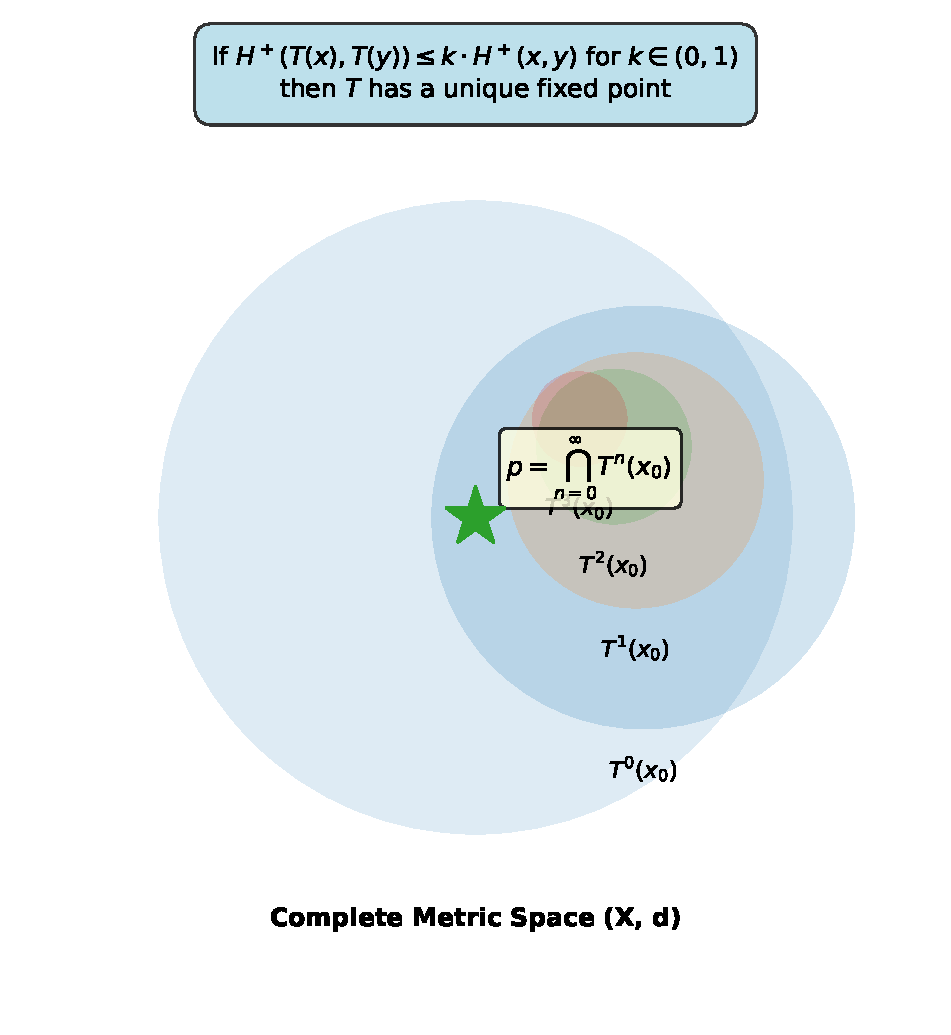
\includegraphics[width=0.8\textwidth]{nadler_theorem}

\end{frame}

\begin{frame}[fragile]
\frametitle{Numerical Example: Nadler's Theorem}

Consider $T: [0,1] \to CB([0,1])$ defined by
\[
T(x) = \left[\frac{x}{3}, \frac{x}{2}\right]
\]

\vspace{0.2cm}

\begin{lstlisting}
import numpy as np

def hausdorff_distance(A, B):
    """Compute Hausdorff distance between intervals"""
    return max(abs(A[0] - B[0]), abs(A[1] - B[1]))

def T(x):
    """Multivalued mapping"""
    return [x/3, x/2]

# Check Nadler condition
x, y = 0.2, 0.5
Tx, Ty = T(x), T(y)
H_dist = hausdorff_distance(Tx, Ty)
k_times_d = 1/3 * abs(x - y)  # Contraction rate k = 1/3

print(f"H(T({x}), T({y})) = {H_dist:.4f}")
print(f"(1/3) * d({x}, {y}) = {k_times_d:.4f}")
print(f"Nadler condition satisfied: {H_dist <= k_times_d}")
\end{lstlisting}

\vspace{0.2cm}

\begin{block}{Fixed Point}
Convergent sequence $\{x_n\}$ converges to $x^* = 0$.
Check: $0 \in [0, 0] = T(0)$ \checkmark
\end{block}

\end{frame}

\begin{frame}
\frametitle{Visualization: Nadler's Contraction}

\centering
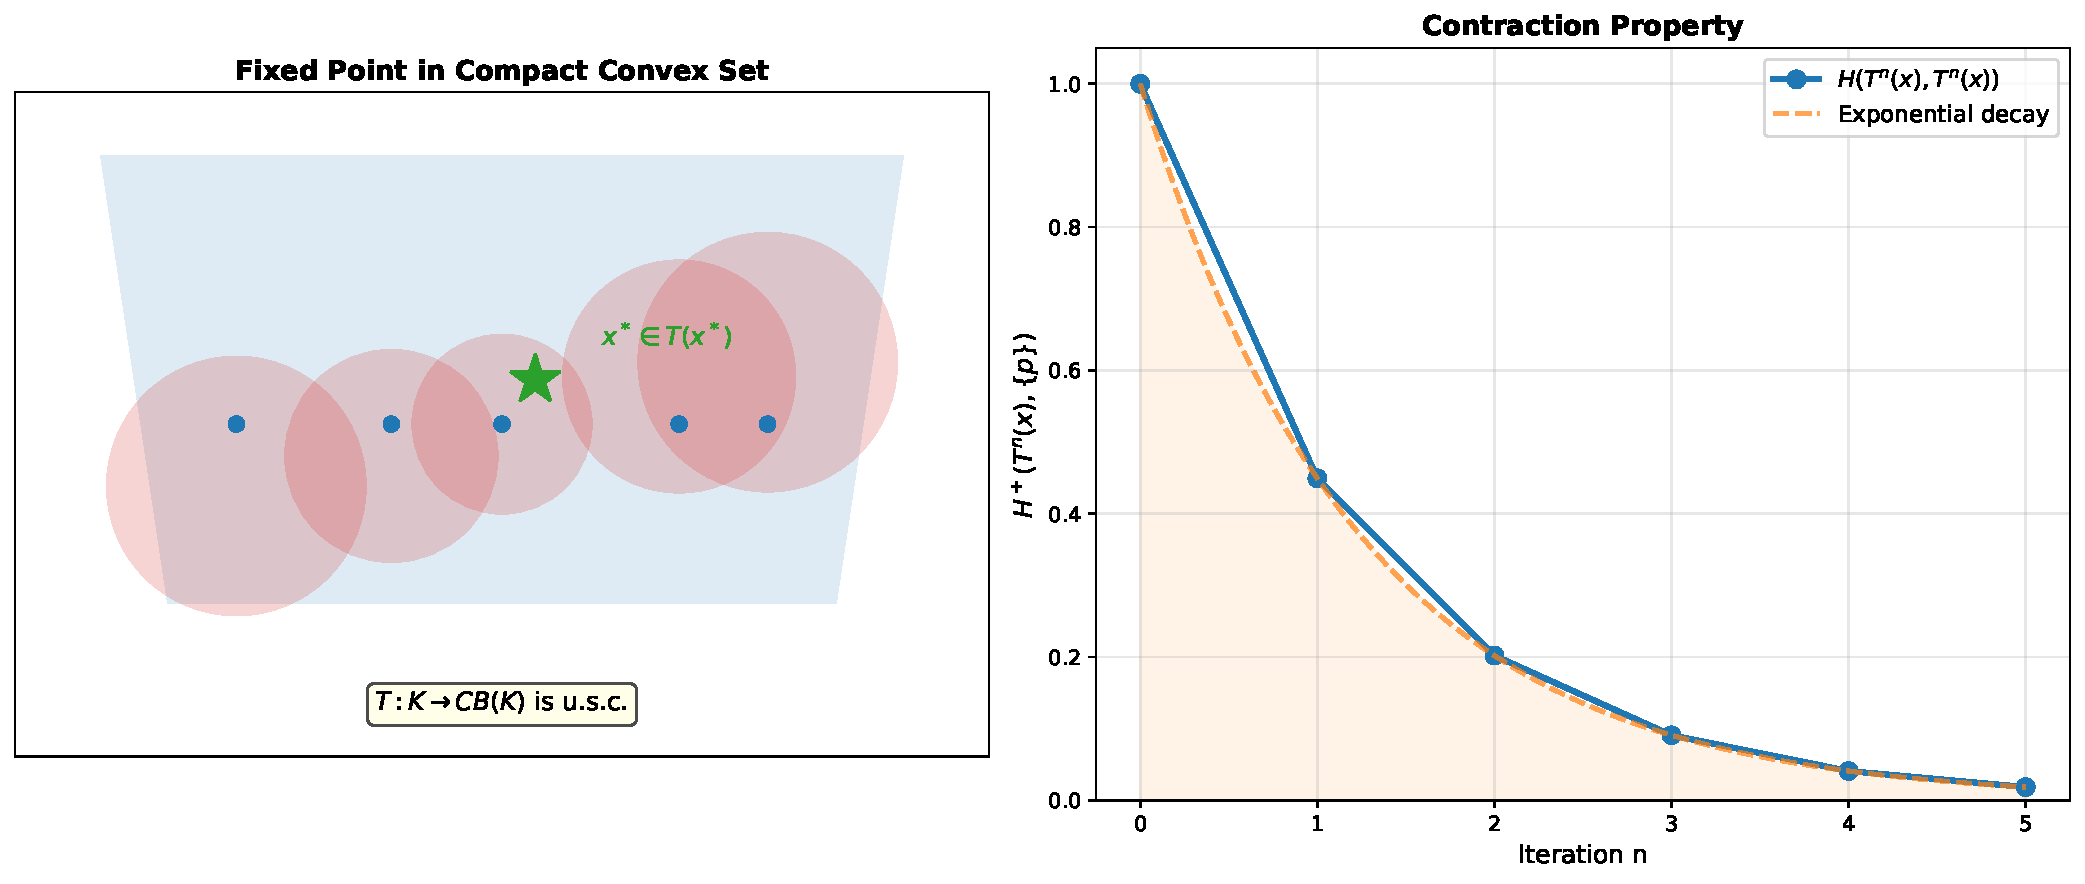
\includegraphics[width=0.9\textwidth]{fixed_point_existence}

\begin{itemize}
    \item \textbf{Left:} Compact convex set $K$ with multivalued mapping showing nested sets
    \item \textbf{Right:} Exponential convergence of iterates to fixed point
\end{itemize}

\end{frame}

% ============================================================================
% SECTION 6: COINCIDENCE AND FIXED POINTS
% ============================================================================

\section{Coincidence and Fixed Points for Multiple Mappings}

\begin{frame}
\frametitle{Coincidence Points}

\begin{definition}
A point $p \in X$ is a \textbf{coincidence point} of mappings $f, g: X \to Y$ if
\[
f(p) = g(p)
\]
\end{definition}

\vspace{0.3cm}

For multivalued mappings $f, g: X \to 2^Y$:
\[
\text{Coincidence point: } f(p) \cap g(p) \neq \emptyset
\]

\vspace{0.3cm}

\centering
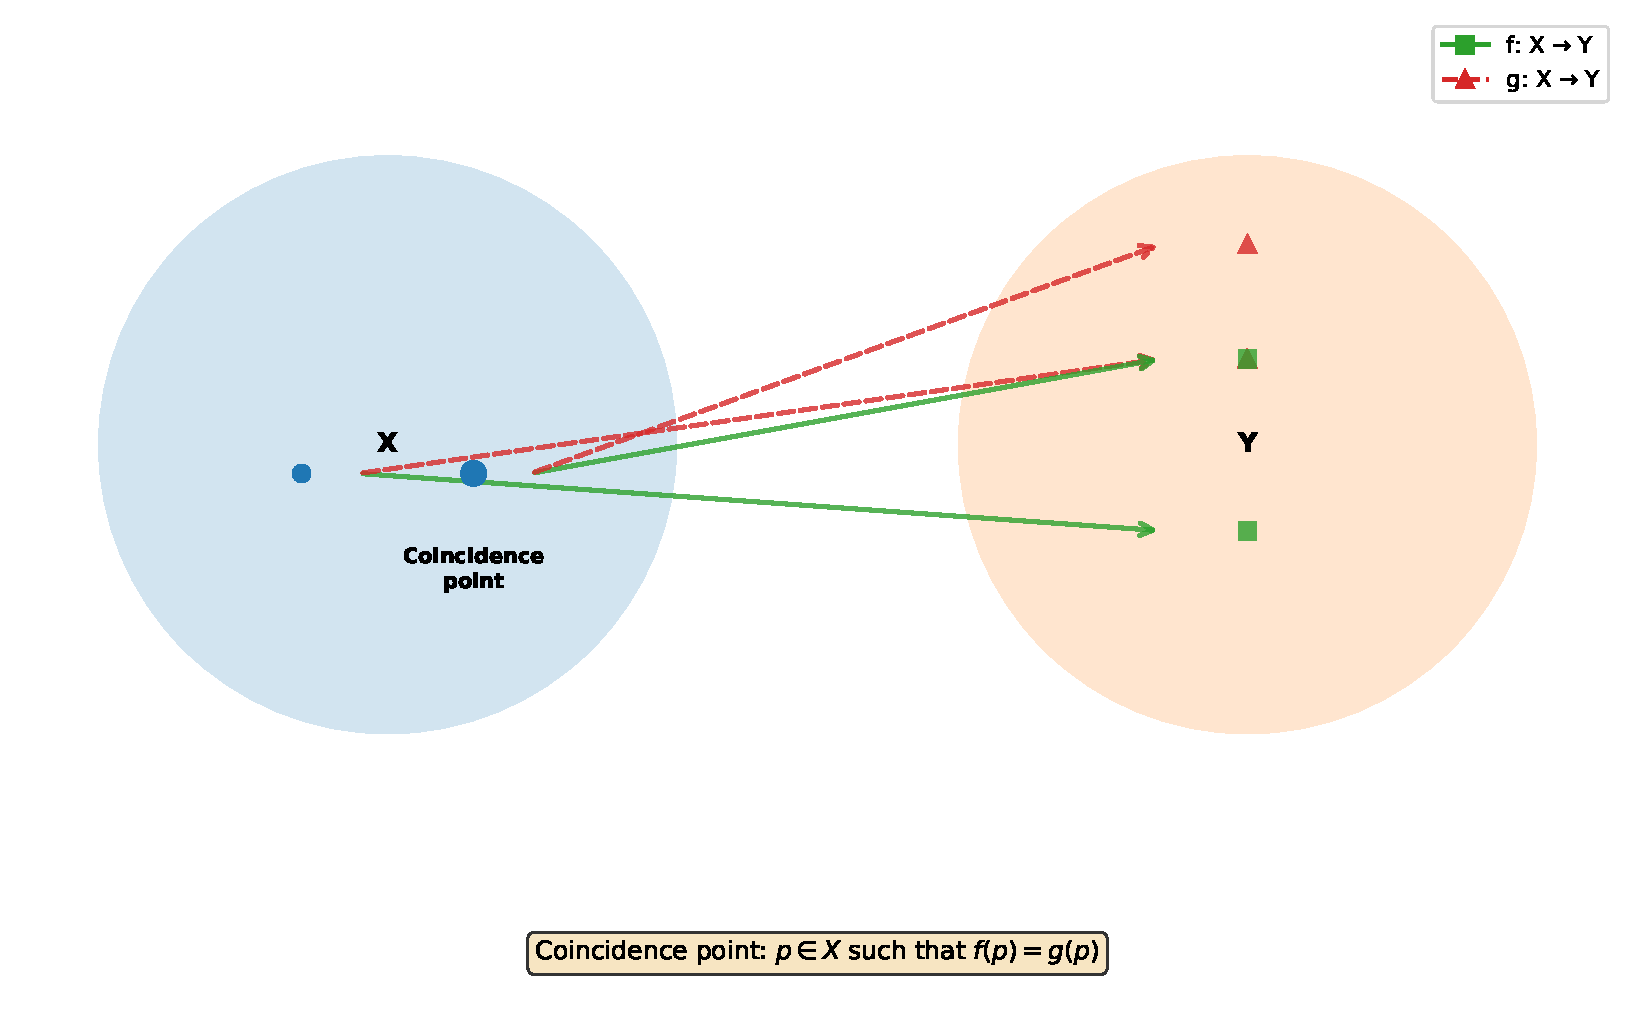
\includegraphics[width=0.85\textwidth]{coincidence_fixed_points}

\vspace{0.2cm}

\textbf{Special Case:} If $g$ is identity, then coincidence points are fixed points of $f$.

\end{frame}

\begin{frame}
\frametitle{Fixed Point Theorems for Two Mappings}

\begin{theorem}[Generalization to Two Mappings]
Let $(X,d)$ be a complete metric space.
Let $S, T: X \to CB(X)$ satisfy the condition:
\[
H(S(x), T(y)) \leq k \cdot d(x,y) \quad \text{for all } x,y \in X
\]
for some $k \in (0,1)$. Then there exists $p \in X$ such that $p \in S(p) \cap T(p)$.
\end{theorem}

\vspace{0.3cm}

\begin{block}{Common Fixed Points}
If both $S$ and $T$ satisfy:
\[
H(S(x), S(y)) \leq k_S \cdot d(x,y), \quad H(T(x), T(y)) \leq k_T \cdot d(x,y)
\]
then they have a common fixed point.
\end{block}

\vspace{0.3cm}

\textbf{Applications:} Variational inequalities, nonlinear integral equations, differential inclusions

\end{frame}

\begin{frame}
\frametitle{Hybrid Mappings and Coincidence}

\begin{definition}
Mappings $f: X \to X$ and $T: X \to 2^X$ are said to have a \textbf{coincidence point} at $p$ if
\[
f(p) \in T(p)
\]
\end{definition}

\vspace{0.3cm}

\begin{theorem}[Coincidence for Hybrid Mappings]
Let $f: X \to X$ be continuous and $T: X \to CB(X)$ be u.s.c. in a compact metric space.
If $H(T(x), T(y)) \leq k \cdot d(f(x), f(y))$ for $k < 1$, then $f$ and $T$ have a coincidence point.
\end{theorem}

\vspace{0.3cm}

\textbf{Key Applications:}
\begin{itemize}
    \item Periodic points of iterative schemes
    \item Common fixed points of commuting families
    \item Solutions to differential inclusions
\end{itemize}

\end{frame}

% ============================================================================
% SECTION 7: ASYMPTOTICALLY CONTRACTIVE MAPPINGS
% ============================================================================

\section{Asymptotically Contractive Multivalued Mappings}

\begin{frame}
\frametitle{Asymptotic Contraction}

\begin{definition}
A multivalued mapping $T: X \to 2^X$ is \textbf{asymptotically I-contractive} if there exist
sequences $\{k_n\}$, $\{\alpha_n\}$ with:
\[
\sum_{n=1}^\infty k_n < \infty, \quad \sum_{n=1}^\infty \alpha_n < \infty
\]
such that for all $x, y \in X$:
\[
H(T^n(x), T^n(y)) \leq k_n \cdot d(x,y) + \alpha_n
\]
\end{definition}

\vspace{0.3cm}

\textbf{Motivation:}
\begin{itemize}
    \item Relaxes strict contraction requirement
    \item Allows error terms that decrease overall
    \item Captures behavior of iterative algorithms with diminishing step sizes
\end{itemize}

\end{frame}

\begin{frame}
\frametitle{Fixed Point Theorem for Asymptotic Contractions}

\begin{theorem}
Let $(X,d)$ be a complete metric space and $T: X \to CB(X)$ asymptotically I-contractive.
If $\sum_{n=1}^\infty k_n < \infty$ and $\sum_{n=1}^\infty \alpha_n < \infty$, then:
\begin{enumerate}
    \item $T$ has a unique fixed point $p$
    \item For any $x_0 \in X$, the Picard iteration $x_{n+1} \in T(x_n)$ converges to $p$
    \item The convergence is exponential
\end{enumerate}
\end{theorem}

\vspace{0.3cm}

\begin{block}{Comparison with Classical Nadler}
\begin{itemize}
    \item Nadler: constant contraction $H(T(x), T(y)) \leq k \cdot d(x,y)$
    \item Asymptotic: varying contraction with summable error $H(T^n(x), T^n(y)) \leq k_n \cdot d(x,y) + \alpha_n$
    \item More flexible for non-stationary iterations
\end{itemize}
\end{block}

\end{frame}

\begin{frame}
\frametitle{Convergence Visualization}

\centering
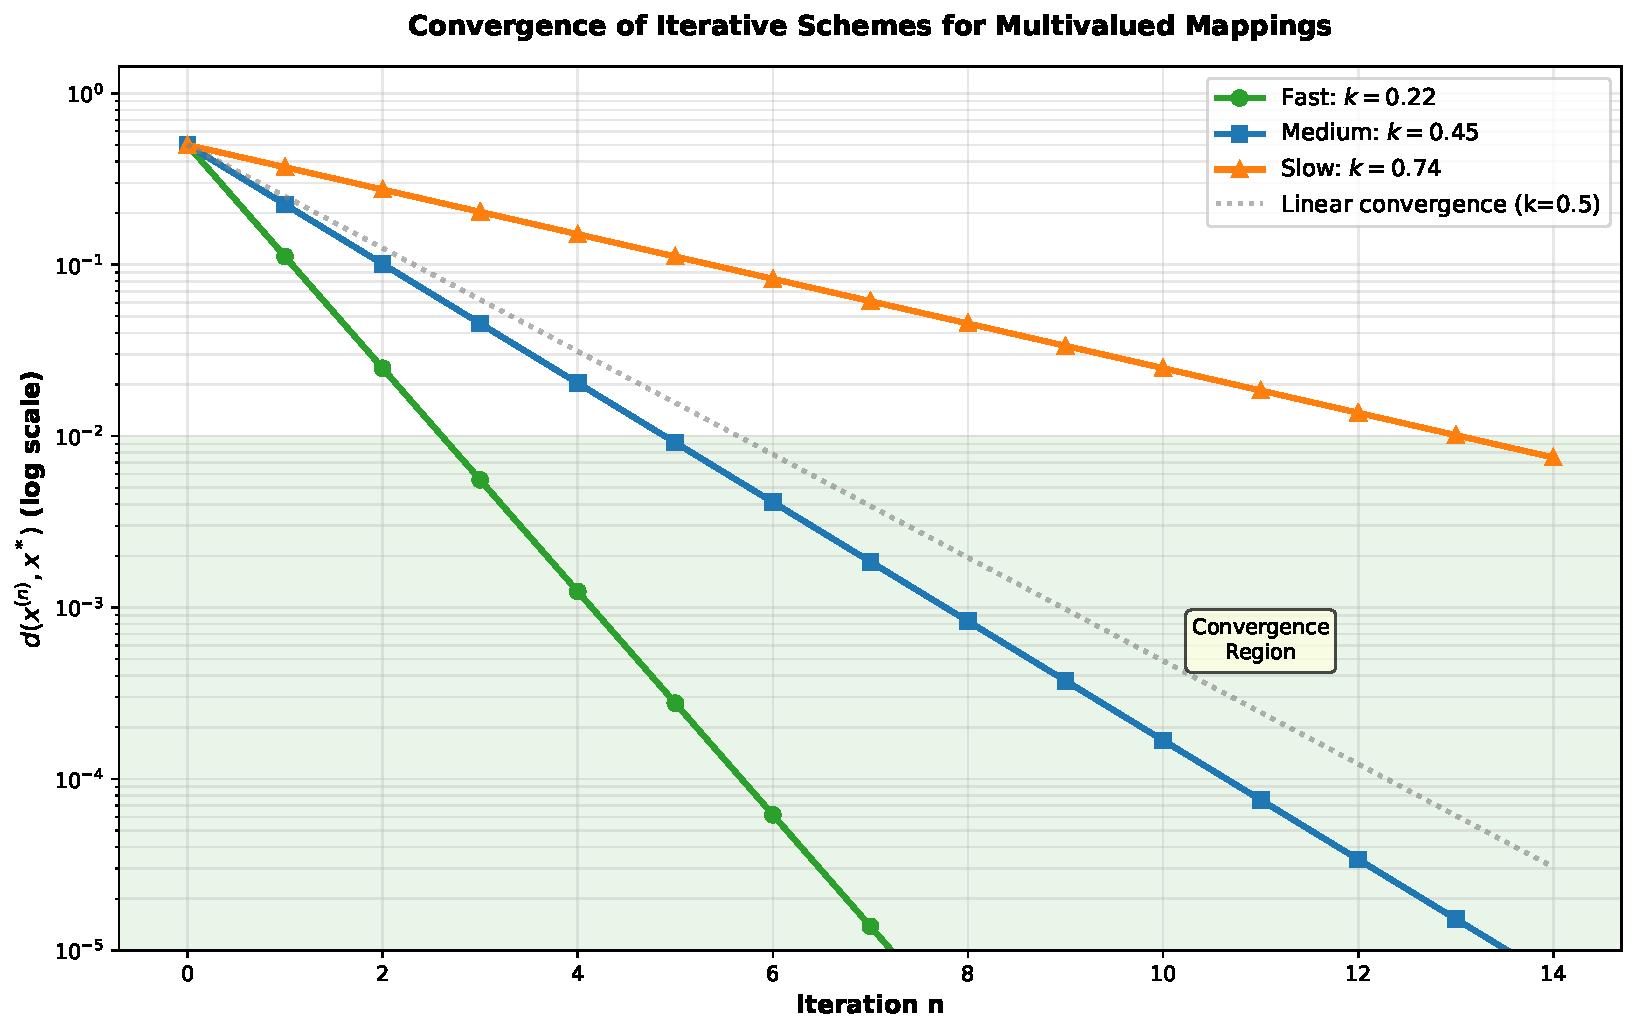
\includegraphics[width=0.9\textwidth]{convergence_iteration}

\begin{itemize}
    \item Different contraction rates $k$ lead to different convergence speeds
    \item Asymptotic setting allows decreasing contraction rates
    \item All converge exponentially to fixed point
\end{itemize}

\end{frame}

% ============================================================================
% SECTION 8: APPLICATIONS
% ============================================================================

\section{Applications and Examples}

\begin{frame}
\frametitle{Applications in Differential Inclusions}

\begin{definition}
A \textbf{differential inclusion} is a generalization of ODEs:
\[
\dot{x}(t) \in F(t, x(t))
\]
where $F$ is a multivalued mapping.
\end{definition}

\vspace{0.3cm}

\textbf{Fixed Point Formulation:}
Using integral formulation:
\[
x(t) = x_0 + \int_0^t f(s, x(s)) \, ds, \quad f(s, x) \in F(s, x)
\]

Define integral operator $T$ on function space:
\[
T(x)(t) = x_0 + \int_0^t F(s, x(s)) \, ds
\]

Then solutions are fixed points of $T$.

\vspace{0.3cm}

\begin{block}{Existence Theorem}
If $F$ is u.s.c. with closed convex values and satisfies growth condition,
then by fixed point theorems, differential inclusion has solution.
\end{block}

\end{frame}

\begin{frame}
\frametitle{Applications in Game Theory}

\begin{block}{Non-Cooperative Games}
Consider strategic game with players choosing from sets $S_i$ (strategy multivalued mappings).
Player payoff: $u_i(s_1, \ldots, s_n)$.
\end{block}

\vspace{0.3cm}

\textbf{Best Response Correspondence:}
\[
BR_i(s_{-i}) = \arg\max_{s_i \in S_i} u_i(s_i, s_{-i})
\]

This is multivalued when multiple strategies maximize utility.

\vspace{0.3cm}

\begin{theorem}[Nash Equilibrium Existence]
If $BR_i$ are u.s.c. with compact convex values, then by Kakutani's/Fan's theorem,
there exists Nash equilibrium $(s_1^*, \ldots, s_n^*)$ such that
$s_i^* \in BR_i(s_{-i}^*)$ for all $i$.
\end{theorem}

\end{frame}

\begin{frame}
\frametitle{Applications in Variational Inequalities}

\begin{problem}
Find $x^* \in K$ such that
\[
\langle Ax^*, y - x^* \rangle \geq 0 \quad \text{for all } y \in K
\]
where $K$ is closed convex and $A$ is possibly multivalued operator.
\end{problem}

\vspace{0.3cm}

\textbf{Multivalued Setting:}
\[
0 \in T(x^*) + N_K(x^*)
\]
where $N_K(x)$ is the normal cone at $x$ in $K$.

\vspace{0.3cm}

\begin{block}{Fixed Point Reduction}
Using resolvent operator: $J_\lambda = (I + \lambda T)^{-1}$, solutions to VI correspond to
fixed points of $J_\lambda$.

This is again a multivalued fixed point problem.
\end{block}

\end{frame}

\begin{frame}
\frametitle{Example: Control Systems}

\begin{problem}
Linear control system:
\[
\dot{x}(t) = Ax(t) + Bu(t), \quad u(t) \in U
\]
where $U$ is a compact constraint set.
\end{problem}

\vspace{0.3cm}

\textbf{Reachable Set:}
Define $R(t) = $ set of all states reachable at time $t$ from initial state $x_0$.

Can be characterized as:
\[
R(t) = \bigcup_{u \in \mathcal{U}} \left\{e^{At}x_0 + \int_0^t e^{A(t-s)}Bu(s) \, ds\right\}
\]

\vspace{0.3cm}

\begin{block}{Fixed Point Perspective}
In phase space, the reachable set evolves under multivalued "flow" map.
Fixed point theorems for multivalued mappings can ensure:
\begin{itemize}
    \item Existence of invariant sets
    \item Periodic orbits in control systems
    \item Stabilization properties
\end{itemize}
\end{block}

\end{frame}

% ============================================================================
% SECTION 9: GENERALIZATIONS AND EXTENSIONS
% ============================================================================

\section{Generalizations and Extensions}

\begin{frame}
\frametitle{Generalizations of Nadler's Theorem}

\begin{theorem}[Assad and Kirk, 1976]
Let $(X,d)$ be a complete metric space and $T: X \to CB(X)$.
If for some $\phi: [0,\infty) \to [0,\infty)$ with $\phi(t) < t$ for $t > 0$:
\[
H(T(x), T(y)) \leq \phi(d(x,y)) \quad \text{for all } x,y \in X
\]
then $T$ has a fixed point.
\end{theorem}

\vspace{0.3cm}

\begin{block}{Other Extensions}
\begin{itemize}
    \item \textbf{Markin:} Weakly contractive multifunctions in Hilbert spaces
    \item \textbf{Smithson:} Contractive multifunctions with point-wise contractive values
    \item \textbf{Reich:} Set-valued nonexpansive mappings
    \item \textbf{Rhoades:} Various types of weak contractions for multivalued maps
\end{itemize}
\end{block}

\end{frame}

\begin{frame}
\frametitle{Extension to b-Metric and Partial Metric Spaces}

\begin{block}{b-Metric Spaces}
Metric $d$ satisfying triangle inequality with constant $s \geq 1$:
\[
d(x,z) \leq s[d(x,y) + d(y,z)]
\]
\end{block}

\begin{theorem}
Fixed point theorems extend to b-metric spaces with Hausdorff metric appropriately modified.
\end{theorem}

\vspace{0.3cm}

\begin{block}{Partial Metric Spaces}
General metric allowing $d(x,x) > 0$ (non-identical elements at distance 0).
\end{block}

\vspace{0.3cm}

\textbf{Current Research:}
\begin{itemize}
    \item Multivalued mappings in metric-like spaces
    \item Fuzzy-valued mappings
    \item Mappings with non-convex values
\end{itemize}

\end{frame}

\begin{frame}
\frametitle{Open Problems and Future Directions}

\begin{itemize}
    \item \textbf{Uniqueness of Fixed Points:} Under what conditions is fixed point unique?

    \item \textbf{Stability Under Perturbations:} How robust are fixed points to small changes in $T$?

    \item \textbf{Global Convergence:} Can we guarantee convergence from any starting point without local assumptions?

    \item \textbf{Computational Methods:} Efficient algorithms for approximating fixed points

    \item \textbf{Multivalued Versions:} Fixed point theory for other problem types (eigenvalue problems, optimization)

    \item \textbf{Applications:} New applications in machine learning, data analysis, uncertainty quantification
\end{itemize}

\end{frame}

% ============================================================================
% SECTION 10: SUMMARY
% ============================================================================

\section{Summary and Key Takeaways}

\begin{frame}
\frametitle{Main Results Summary}

\begin{table}[h]
\centering
\small
\begin{tabular}{|l|l|l|}
\hline
\textbf{Theorem} & \textbf{Conditions} & \textbf{Conclusion} \\
\hline
\textbf{Fan (1952)} & u.s.c., closed convex values, & Fixed point \\
& compact domain & in $K$ \\
\hline
\textbf{Himmelberg (1972)} & u.s.c., closed convex, & Fixed point \\
& compact range & exists \\
\hline
\textbf{Nadler (1969)} & $H(T(x), T(y)) \leq k \cdot d(x,y)$ & Unique fixed \\
& $k < 1$ on complete space & point \\
\hline
\textbf{Asymptotic} & $H(T^n(x), T^n(y))$ & Unique fixed \\
\textbf{Contraction} & $\leq k_n d(x,y) + \alpha_n$ & point, exponential \\
& $\sum k_n, \sum \alpha_n < \infty$ & convergence \\
\hline
\end{tabular}
\end{table}

\end{frame}

\begin{frame}
\frametitle{Key Concepts}

\begin{itemize}
    \item \textbf{Multivalued Mapping:} $T: X \to 2^X$ maps points to sets

    \item \textbf{Fixed Point:} $x^* \in T(x^*)$ (set membership, not equality)

    \item \textbf{Hausdorff Metric:} $H(A,B)$ measures distance between sets

    \item \textbf{Upper Semicontinuity:} Natural continuity notion for multifunctions

    \item \textbf{Contraction:} $H(T(x), T(y)) \leq k \cdot d(x,y)$ for $k < 1$

    \item \textbf{Topological Methods:} Compactness + convexity + continuity guarantee fixed point

    \item \textbf{Metric Methods:} Contractions guarantee unique fixed point with convergence
\end{itemize}

\end{frame}

\begin{frame}
\frametitle{Connections to Other Topics}

\begin{itemize}
    \item \textbf{Differential Equations:} Solutions via integral reformulation as fixed points

    \item \textbf{Optimization:} Variational inequalities reduce to fixed point problems

    \item \textbf{Game Theory:} Nash equilibria are fixed points of best response mappings

    \item \textbf{Economics:} Market equilibrium, general equilibrium theory

    \item \textbf{Control Theory:} Reachable sets, invariant sets, stabilization

    \item \textbf{Numerical Analysis:} Iteration schemes, convergence analysis

    \item \textbf{Topology:} Degree theory, index theory, homotopy
\end{itemize}

\end{frame}

\begin{frame}
\frametitle{Resources and Further Reading}

\begin{block}{Key References}
\begin{itemize}
    \item Pathak, H. K. (2018). \textit{Introduction to Nonlinear Analysis and Fixed Point Theory}. Springer.

    \item Aubin, J. P., \& Frankowska, H. (2009). \textit{Set-Valued Analysis}. Birkhäuser.

    \item Denkowski, Z., Migórski, S., \& Papageorgiou, N. S. (2003). \textit{An Introduction to Nonlinear Analysis: Theory}. Springer.
\end{itemize}
\end{block}

\vspace{0.3cm}

\begin{block}{Topics for Deeper Study}
\begin{itemize}
    \item Measure of noncompactness and condensing multivalued mappings
    \item Fixed points for mappings with non-convex values
    \item Multivalued versions of Mann and Ishikawa iterations
    \item Differential inclusions and their solutions
\end{itemize}
\end{block}

\end{frame}

\begin{frame}[allowframebreaks]
\frametitle{Conclusion}

\begin{itemize}
    \item Multivalued mappings extend classical fixed point theory to set-valued functions

    \item The Hausdorff-Pompeu metric provides the natural framework

    \item Two main approaches:
    \begin{itemize}
        \item \textbf{Topological:} Compactness + continuity + convexity (Fan, Himmelberg)
        \item \textbf{Metric:} Contractions with complete space (Nadler)
    \end{itemize}

    \item Rich applications in:
    \begin{itemize}
        \item Differential inclusions
        \item Variational inequalities
        \item Game theory and economics
        \item Control theory
    \end{itemize}

    \item Active area of research with numerous generalizations and extensions

    \item Bridges pure mathematics with practical applications
\end{itemize}

\vspace{0.5cm}

\centering
\Large \textbf{Thank You!}

\end{frame}

\end{document}
